\documentclass[11pt,]{article}
\usepackage{lmodern}
\usepackage{amssymb,amsmath}
\usepackage{ifxetex,ifluatex}
\usepackage{fixltx2e} % provides \textsubscript
\ifnum 0\ifxetex 1\fi\ifluatex 1\fi=0 % if pdftex
  \usepackage[T1]{fontenc}
  \usepackage[utf8]{inputenc}
\else % if luatex or xelatex
  \ifxetex
    \usepackage{mathspec}
  \else
    \usepackage{fontspec}
  \fi
  \defaultfontfeatures{Ligatures=TeX,Scale=MatchLowercase}
\fi
% use upquote if available, for straight quotes in verbatim environments
\IfFileExists{upquote.sty}{\usepackage{upquote}}{}
% use microtype if available
\IfFileExists{microtype.sty}{%
\usepackage{microtype}
\UseMicrotypeSet[protrusion]{basicmath} % disable protrusion for tt fonts
}{}
\usepackage[margin = 1.5in]{geometry}
\usepackage{hyperref}
\PassOptionsToPackage{usenames,dvipsnames}{color} % color is loaded by hyperref
\hypersetup{unicode=true,
            pdftitle={Integration Among US Banks: Rerun},
            pdfauthor={Abhinav Anand and John Cotter},
            colorlinks=true,
            linkcolor=blue,
            citecolor=magenta,
            urlcolor=red,
            breaklinks=true}
\urlstyle{same}  % don't use monospace font for urls
\usepackage{longtable,booktabs}
\usepackage{graphicx,grffile}
\makeatletter
\def\maxwidth{\ifdim\Gin@nat@width>\linewidth\linewidth\else\Gin@nat@width\fi}
\def\maxheight{\ifdim\Gin@nat@height>\textheight\textheight\else\Gin@nat@height\fi}
\makeatother
% Scale images if necessary, so that they will not overflow the page
% margins by default, and it is still possible to overwrite the defaults
% using explicit options in \includegraphics[width, height, ...]{}
\setkeys{Gin}{width=\maxwidth,height=\maxheight,keepaspectratio}
\IfFileExists{parskip.sty}{%
\usepackage{parskip}
}{% else
\setlength{\parindent}{0pt}
\setlength{\parskip}{6pt plus 2pt minus 1pt}
}
\setlength{\emergencystretch}{3em}  % prevent overfull lines
\providecommand{\tightlist}{%
  \setlength{\itemsep}{0pt}\setlength{\parskip}{0pt}}
\setcounter{secnumdepth}{0}
% Redefines (sub)paragraphs to behave more like sections
\ifx\paragraph\undefined\else
\let\oldparagraph\paragraph
\renewcommand{\paragraph}[1]{\oldparagraph{#1}\mbox{}}
\fi
\ifx\subparagraph\undefined\else
\let\oldsubparagraph\subparagraph
\renewcommand{\subparagraph}[1]{\oldsubparagraph{#1}\mbox{}}
\fi

%%% Use protect on footnotes to avoid problems with footnotes in titles
\let\rmarkdownfootnote\footnote%
\def\footnote{\protect\rmarkdownfootnote}

%%% Change title format to be more compact
\usepackage{titling}

% Create subtitle command for use in maketitle
\newcommand{\subtitle}[1]{
  \posttitle{
    \begin{center}\large#1\end{center}
    }
}

\setlength{\droptitle}{-2em}

  \title{Integration Among US Banks: Rerun}
    \pretitle{\vspace{\droptitle}\centering\huge}
  \posttitle{\par}
    \author{Abhinav Anand and John Cotter}
    \preauthor{\centering\large\emph}
  \postauthor{\par}
      \predate{\centering\large\emph}
  \postdate{\par}
    \date{2019/03/05}

\linespread{1.25}
\usepackage{amsmath}

\begin{document}
\maketitle

\section{Explantory Power of
Eigenvectors}\label{explantory-power-of-eigenvectors}

\begin{center}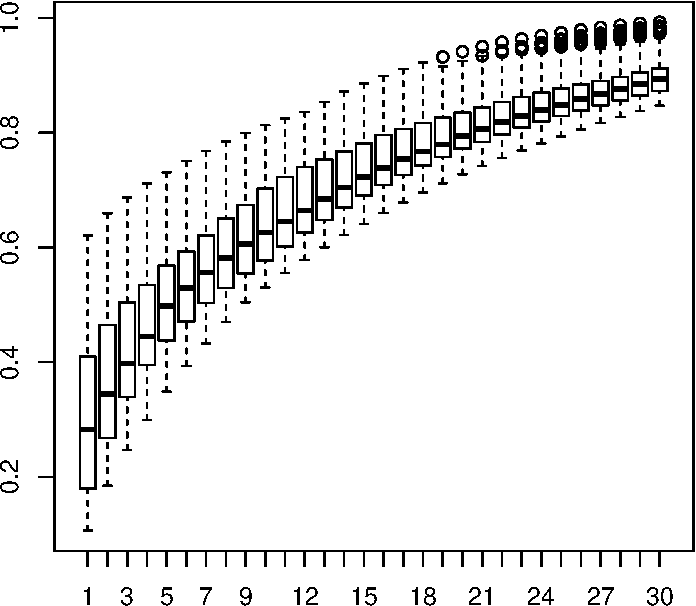
\includegraphics{AC_US_Bank_Int_Results_1_files/figure-latex/expl_power_eig_vec-1} \end{center}

\section{Median US Bank Integration}\label{median-us-bank-integration}

\subsection{Trends}\label{trends}

\subsubsection{Tables}\label{tables}

\begin{longtable}[]{@{}lrrrr@{}}
\caption{Pre 2005 trend}\tabularnewline
\toprule
term & estimate & std.error & statistic & p.value\tabularnewline
\midrule
\endfirsthead
\toprule
term & estimate & std.error & statistic & p.value\tabularnewline
\midrule
\endhead
(Intercept) & 0.4635295 & 0.0145597 & 31.836396 & 0\tabularnewline
Qtr\_num & 0.0021438 & 0.0002506 & 8.553111 & 0\tabularnewline
\bottomrule
\end{longtable}

\begin{longtable}[]{@{}lrrrr@{}}
\caption{Post 2005 trend}\tabularnewline
\toprule
term & estimate & std.error & statistic & p.value\tabularnewline
\midrule
\endfirsthead
\toprule
term & estimate & std.error & statistic & p.value\tabularnewline
\midrule
\endhead
(Intercept) & 0.5097026 & 0.0110443 & 46.1506284 &
0.0000000\tabularnewline
Qtr\_num & -0.0000520 & 0.0003542 & -0.1468808 &
0.8838543\tabularnewline
\bottomrule
\end{longtable}

\begin{longtable}[]{@{}lrrrr@{}}
\caption{Systemic banks trend}\tabularnewline
\toprule
term & estimate & std.error & statistic & p.value\tabularnewline
\midrule
\endfirsthead
\toprule
term & estimate & std.error & statistic & p.value\tabularnewline
\midrule
\endhead
(Intercept) & 0.5102046 & 0.0521200 & 9.789035 &
0.0000000\tabularnewline
Qtr\_num & 0.0016673 & 0.0006166 & 2.703940 & 0.0094509\tabularnewline
\bottomrule
\end{longtable}

\begin{longtable}[]{@{}lrrrr@{}}
\caption{Systemic banks trend pre 2005}\tabularnewline
\toprule
term & estimate & std.error & statistic & p.value\tabularnewline
\midrule
\endfirsthead
\toprule
term & estimate & std.error & statistic & p.value\tabularnewline
\midrule
\endhead
(Intercept) & 0.5362147 & 0.0256320 & 20.91975 & 0e+00\tabularnewline
Qtr\_num & 0.0022427 & 0.0004026 & 5.57005 & 2e-07\tabularnewline
\bottomrule
\end{longtable}

\begin{longtable}[]{@{}lrrrr@{}}
\caption{Systemic banks trend post 2005}\tabularnewline
\toprule
term & estimate & std.error & statistic & p.value\tabularnewline
\midrule
\endfirsthead
\toprule
term & estimate & std.error & statistic & p.value\tabularnewline
\midrule
\endhead
(Intercept) & 0.5336732 & 0.0393933 & 13.547308 &
0.0000000\tabularnewline
Qtr\_num & 0.0026014 & 0.0015051 & 1.728382 & 0.0904851\tabularnewline
\bottomrule
\end{longtable}

\begin{longtable}[]{@{}lrrrr@{}}
\toprule
term & estimate & std.error & statistic & p.value\tabularnewline
\midrule
\endhead
(Intercept) & 0.4357173 & 0.101771 & 4.281352 & 0.0000884\tabularnewline
Qtr\_num & 0.0034857 & 0.001244 & 2.801916 & 0.0073036\tabularnewline
\bottomrule
\end{longtable}

\subsubsection{Plots}\label{plots}

\begin{center}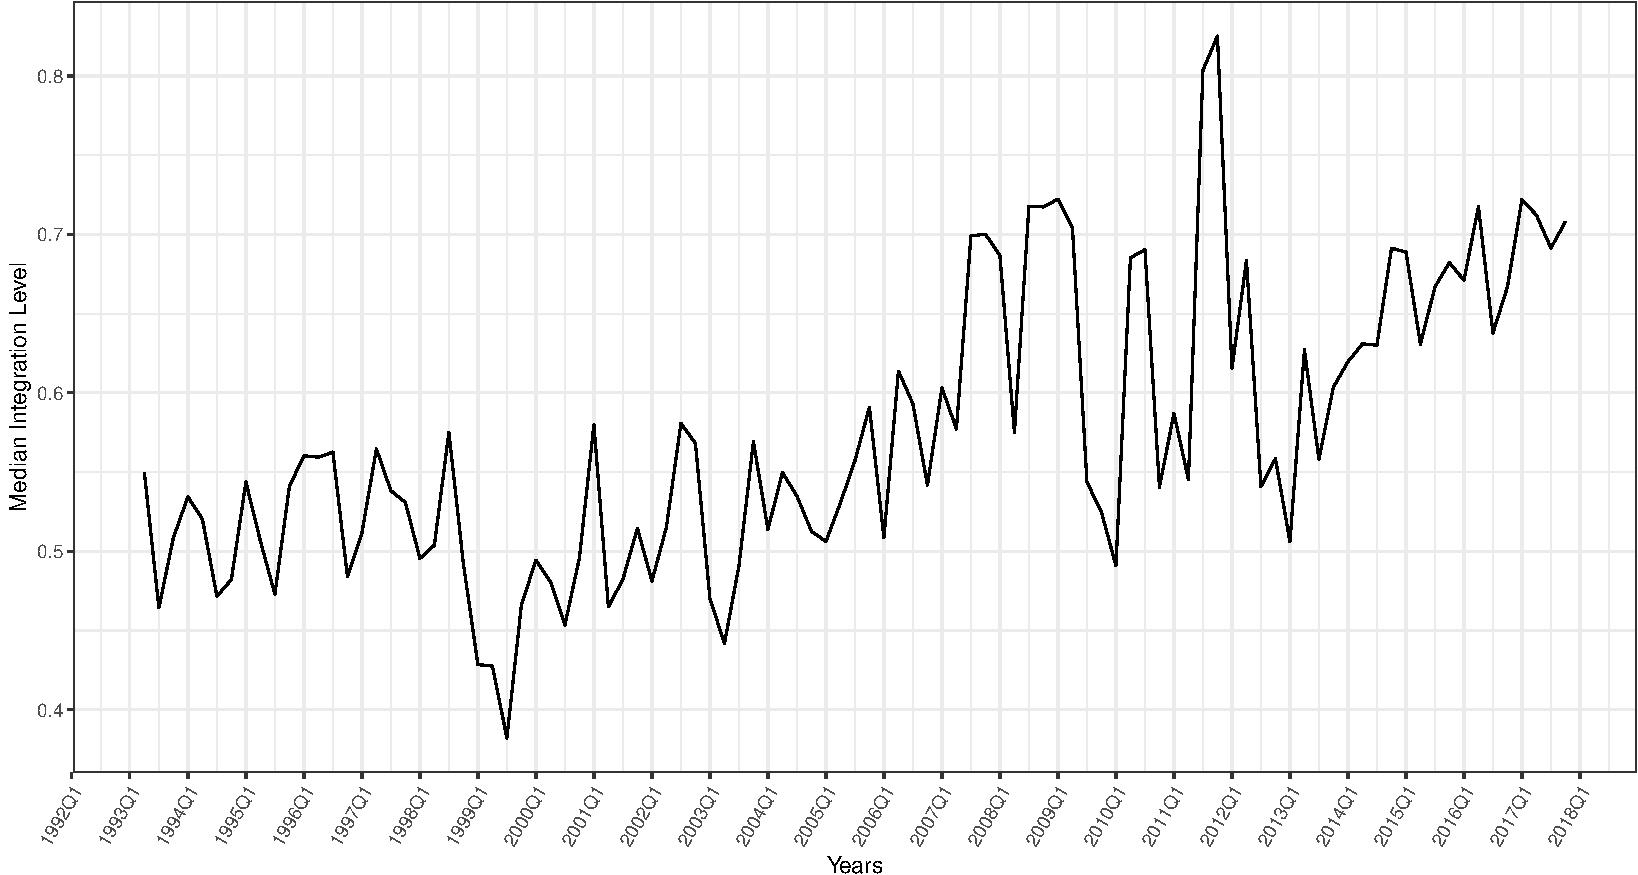
\includegraphics{AC_US_Bank_Int_Results_1_files/figure-latex/med_US_bank_int-1} \end{center}

\begin{center}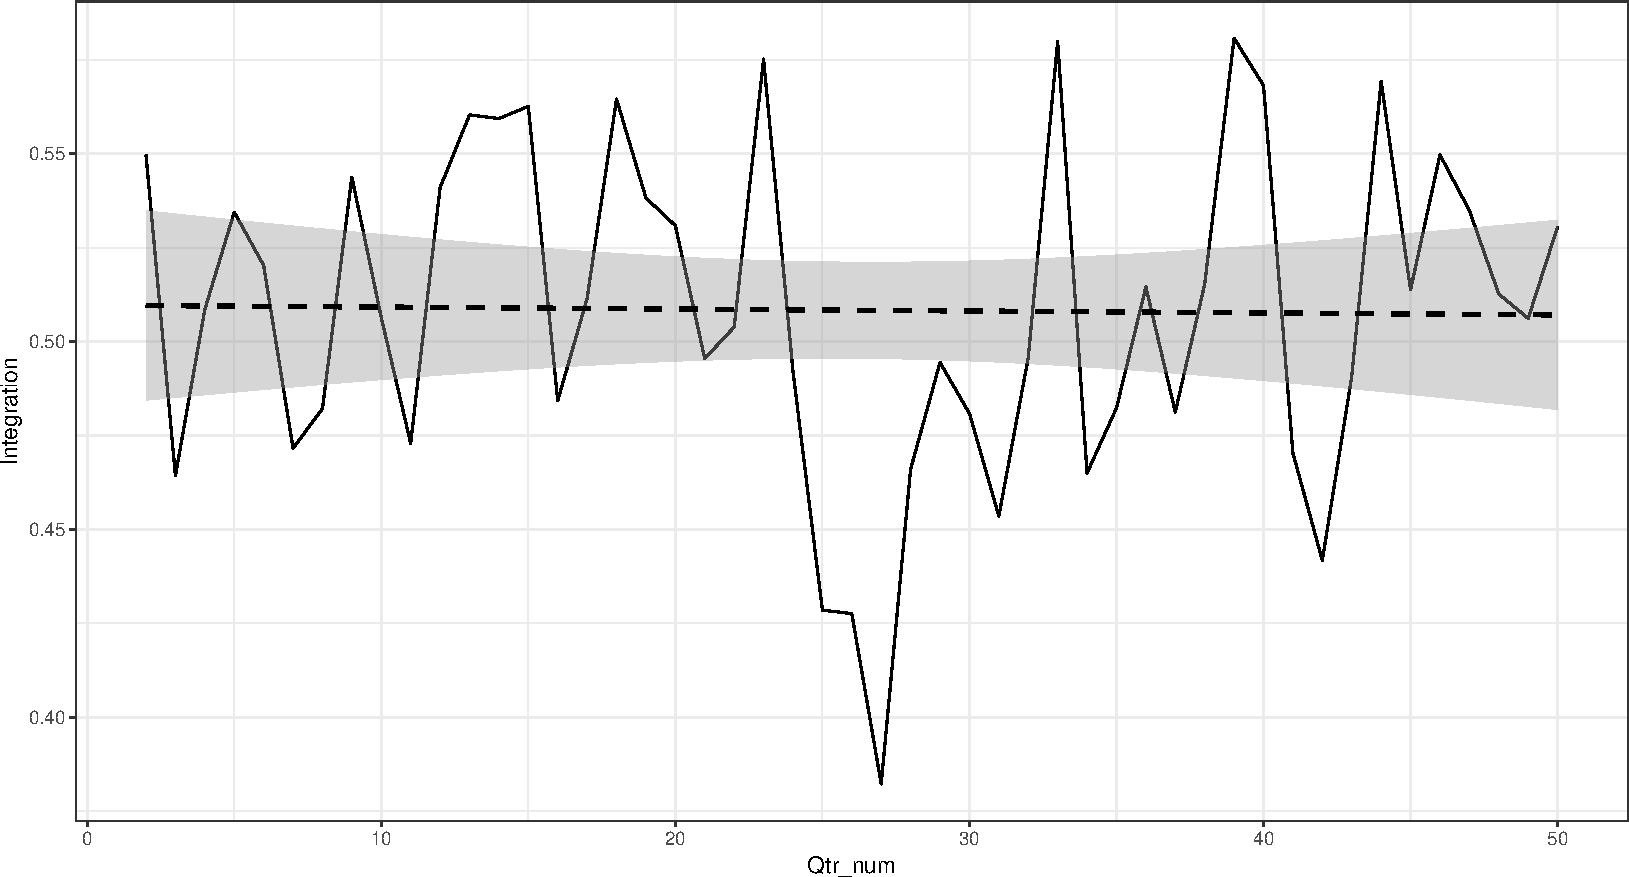
\includegraphics{AC_US_Bank_Int_Results_1_files/figure-latex/med_US_bank_int-2} \end{center}

\begin{center}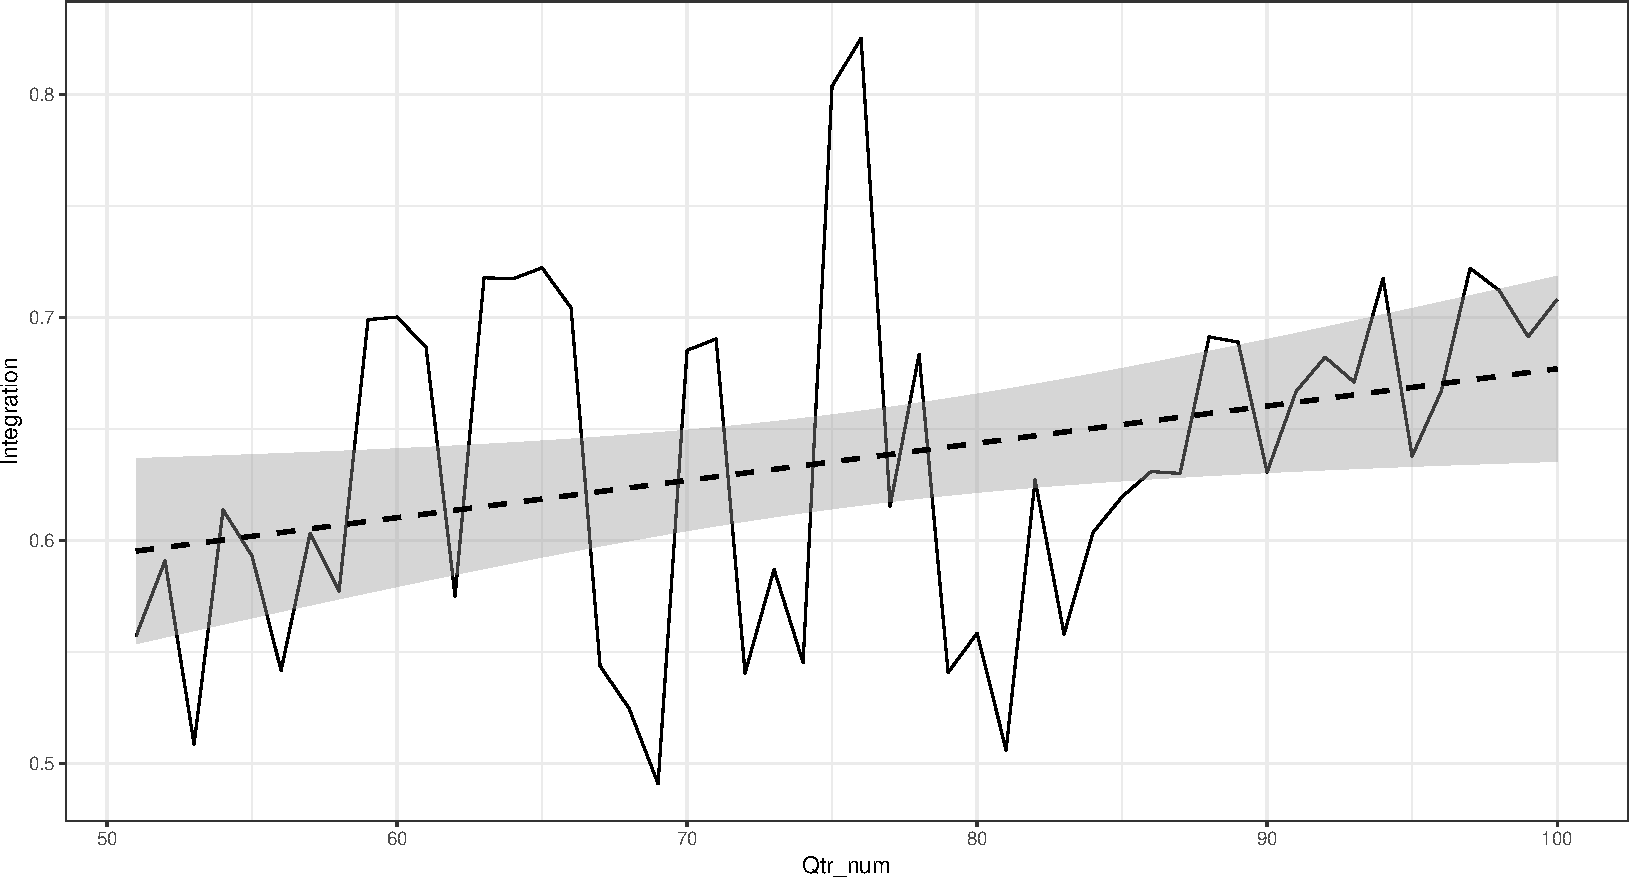
\includegraphics{AC_US_Bank_Int_Results_1_files/figure-latex/med_US_bank_int-3} \end{center}

\begin{center}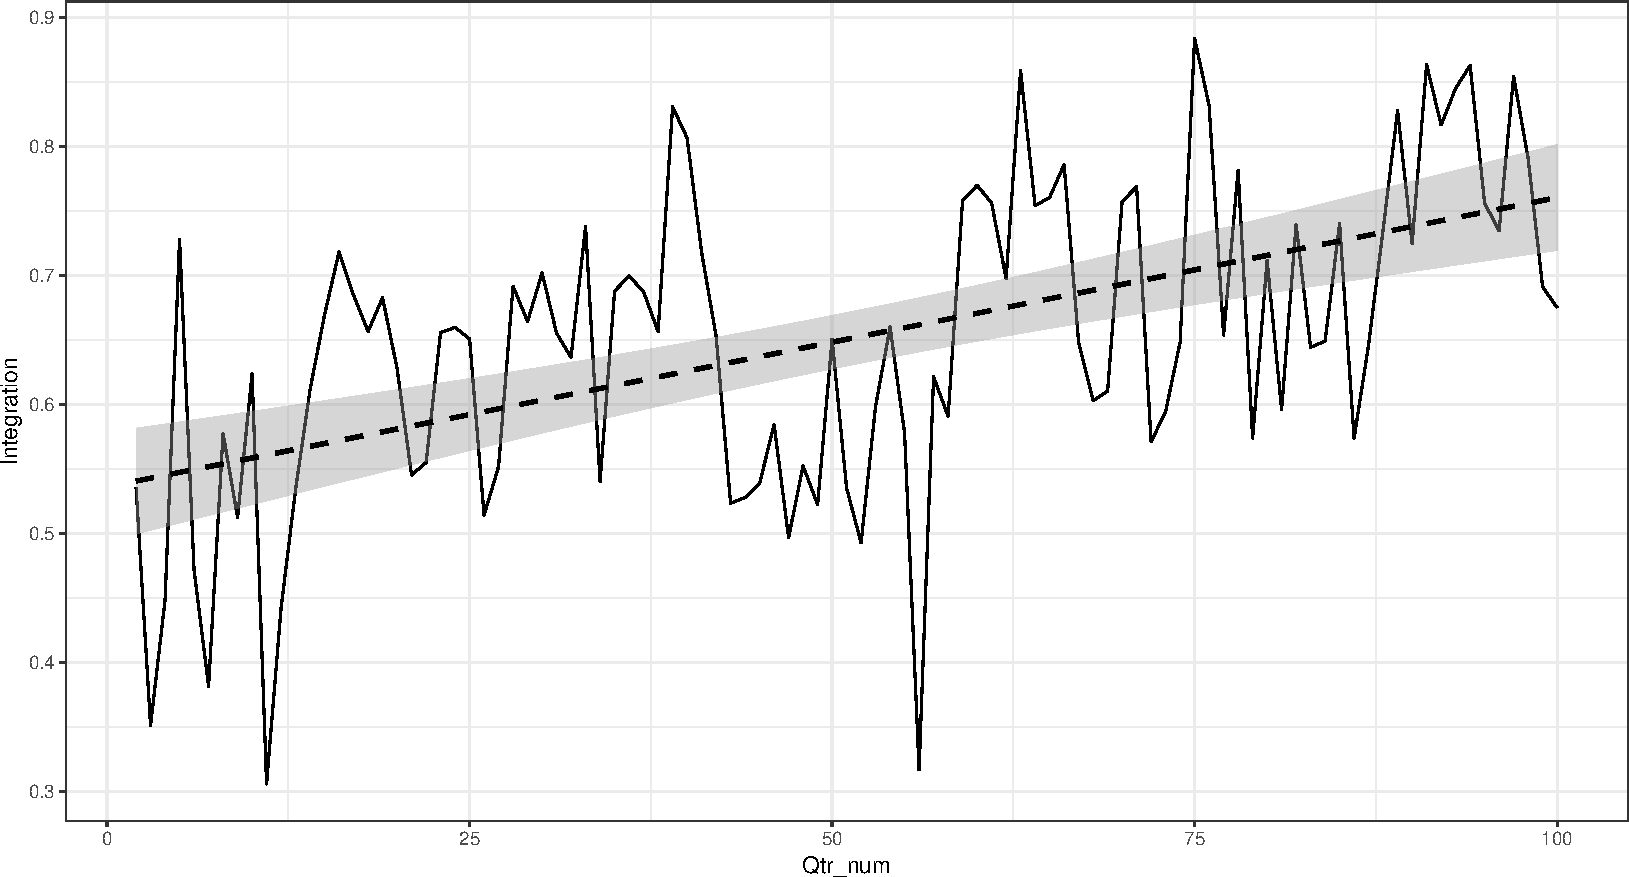
\includegraphics{AC_US_Bank_Int_Results_1_files/figure-latex/med_US_bank_int-4} \end{center}

\begin{center}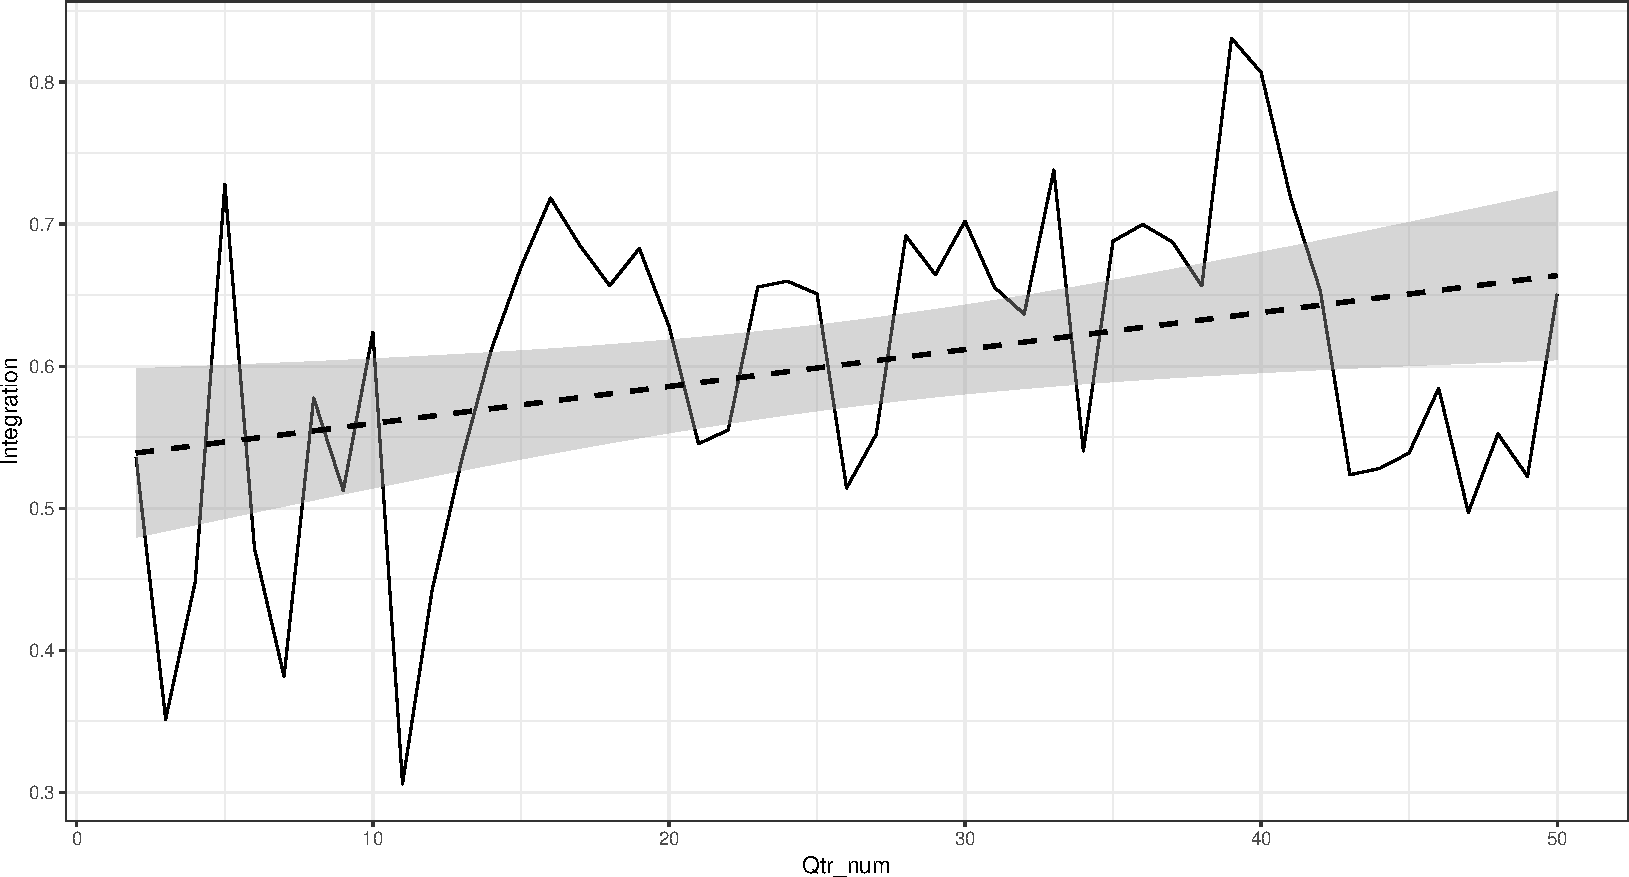
\includegraphics{AC_US_Bank_Int_Results_1_files/figure-latex/med_US_bank_int-5} \end{center}

\begin{center}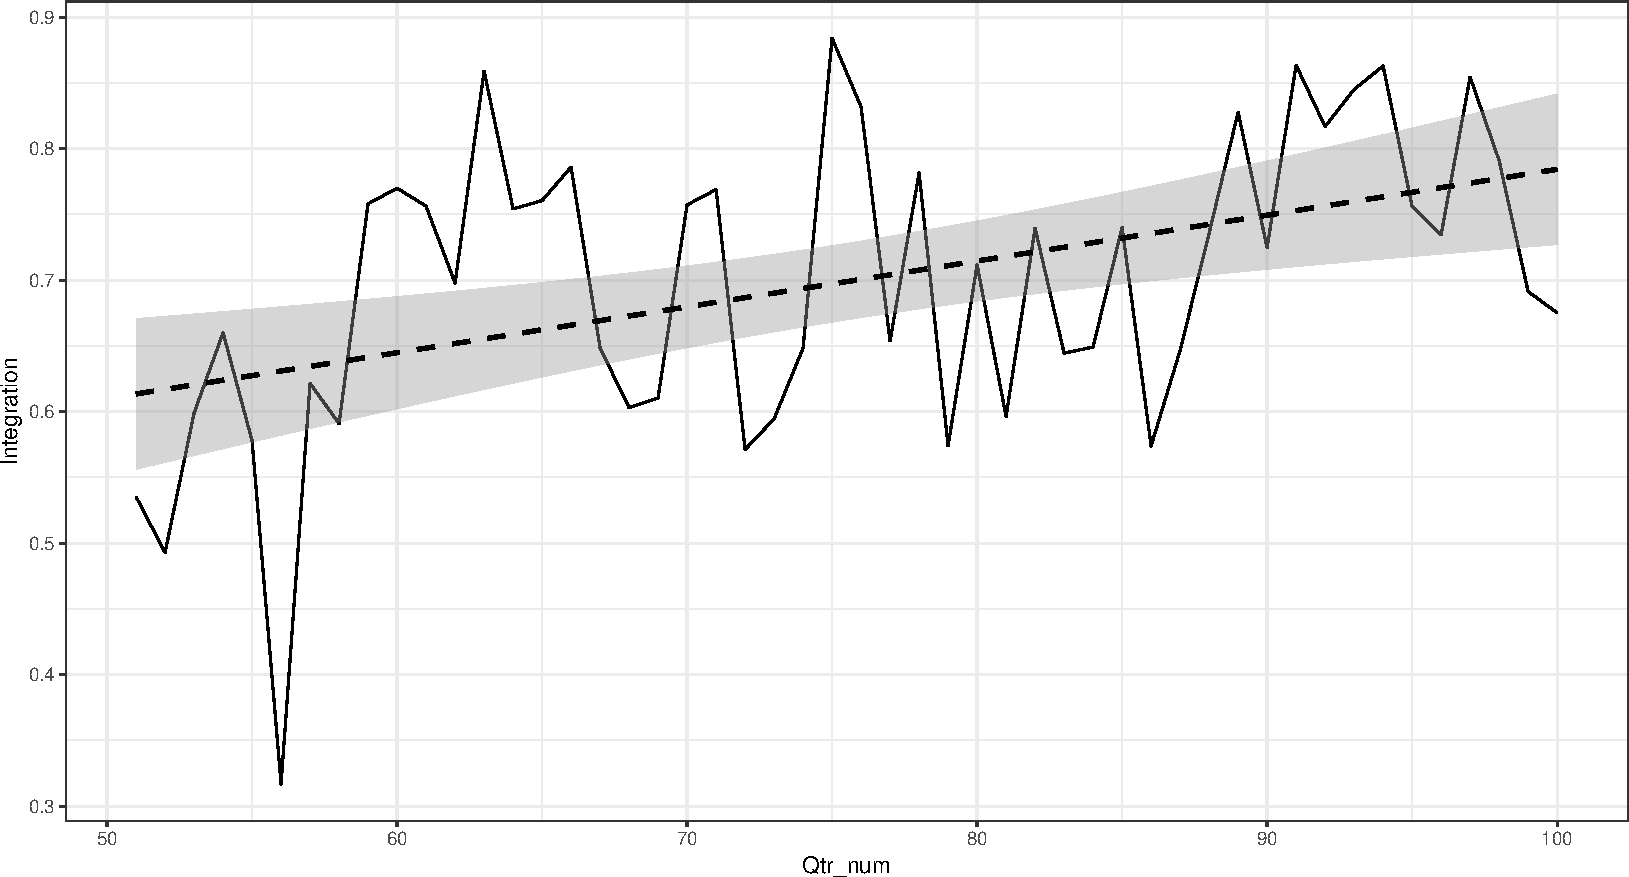
\includegraphics{AC_US_Bank_Int_Results_1_files/figure-latex/med_US_bank_int-6} \end{center}

\section{Empirical Distribution of US Bank
Integration}\label{empirical-distribution-of-us-bank-integration}

\begin{center}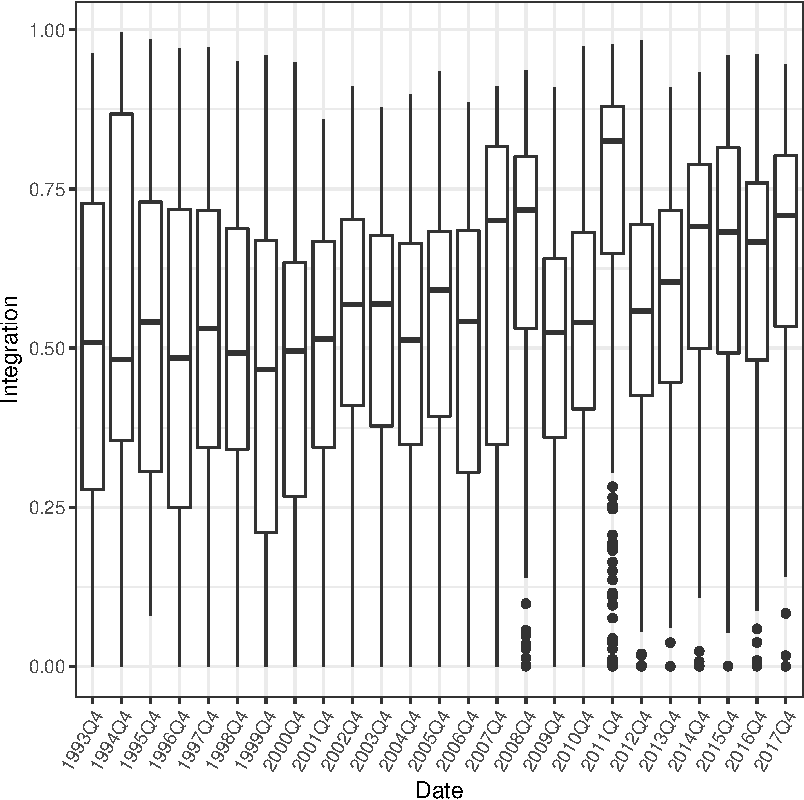
\includegraphics{AC_US_Bank_Int_Results_1_files/figure-latex/emp_distr_US_bank_int-1} \end{center}

\section{Crises}\label{crises}

\begin{longtable}[]{@{}lrrrr@{}}
\toprule
term & estimate & std.error & statistic & p.value\tabularnewline
\midrule
\endhead
(Intercept) & 0.4635592 & 0.0147994 & 31.322849 &
0.0000000\tabularnewline
Qtr\_num & 0.0018850 & 0.0002677 & 7.042690 & 0.0000000\tabularnewline
GR & 0.1078591 & 0.0171983 & 6.271495 & 0.0000000\tabularnewline
EZ & 0.0609390 & 0.0339866 & 1.793030 & 0.0761505\tabularnewline
\bottomrule
\end{longtable}

\section{Panel Estimation}\label{panel-estimation}


\end{document}
